%---------- Quarto Capitulo ----------
\chapter{Resultados e Discussões}
\label{chap:resul}

Os resultados obtidos com o desenvolvimento deste trabalho não realizaram completamente o objetivo proposto neste projeto. As possíveis causas e soluções propostas serão comentadas mais detalhadamente na conclusão deste relatório, por enquanto nos limitaremos a relatar os resultados apresentados e discutir seus significados.

Após vários experimentos com diferentes materiais citados no desenvolvimento chegamos à um modelo final, utilizando a PCI. Com esta configuração pudemos diminuir as variáveis do projeto, trazendo mais estabilidade, porém, como veremos a seguir, não foi o suficiente.

O modelo final do projeto será apresentado na figura 12.

\begin{figure}[!h]
	\centering
	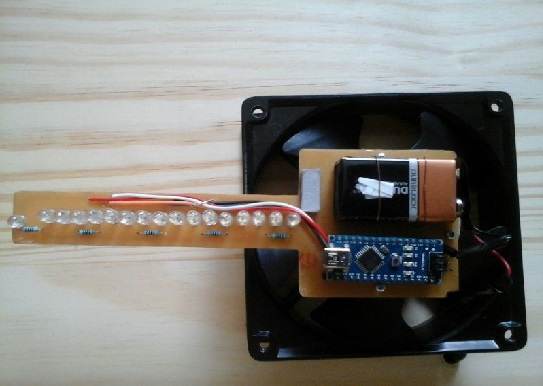
\includegraphics{./modelo_final.jpg}
	\caption[Modelo final do projeto]{Modelo final do projeto}
	\label{fig:modelo_final}
\end{figure}

Utilizando este modelo, foi possível obter um ótimo resultado estético no projeto. A placa e o motor, juntos com a bateria para alimentação dos componentes eletrônicos, encaixaram perfeitamente no hardware desenvolvido pela equipe. Porém, devido à limitações físicas, não foi possível combinar com sucesso a programação do software com o que foi construído. O algoritmo desenvolvido para o funcionamento do relógio funciona perfeitamente se as limitações do hardware forem desconsideradas, e pode ser usado em novos projetos.

Juntando as duas partes do trabalho (software e hardware) foi possível visualizar os ponteiros e a borda do relógio, entretanto, os ponteiros não ficaram fixos na posição em que deveriam estar, pois o número de rotações por minuto do motor estava variando de acordo com as condições físicas do relógio.

Realizando vários testes empíricos foi possível observar que o software funcionou de maneira correta e que a variável que não estava com o comportamento esperado era o número de rotações por minuto. A base do motor não estava completamente fixa, causando uma pequena trepidação em todo o sistema, a potência do motor era muito grande para que houvesse a estabilidade desejada. Na próxima secção deste trabalho serão apresentadas as conclusões da equipe a respeito das soluções para o problema.
